\iffalse \bibliography{include/backmatter/magnus,include/backmatter/philip} \fi
\chapter{Background} \label{sect:background} 
In this section we introduce technological concepts related to this study.
%---------------------------------------------------%
\section{Cyber Physical Systems}
%compact middle-ware OpenDaVINCI written in standard C++, can be used on a variety of POSIX OS. we use ODV to have a lean, portable and high-performance hardware and OS abstraction layer for typical programming idioms like concurrency, data storage and communication. %control, computing, communications 

A cyber physical system (CPS) interacts with the world, sensing their surroundings by using embedded sensors, actuators and processors. These sensors, atuators and processors communicate and collaborate with each other to support real-time, guaranteed performance in safety critical applications \cite{sidcyber}. Applications for CPSs span multiple domains including healthcare (robotic surgery), transportation (autonomous vehicles), agriculture, energy, and home automation to name a few. In the transportation domain for CPSs, autonomous vehicles, also called self-driving vehicles, are vehicles that operate without requiring human input. The intelligent behaviour of a self-driving vehicle include trajectory generation, lane following, lane keeping and intersection handling \cite{sidcyber}. These are some of the computational responsibilities of a CPS for driver-less vehicles.\\ 

The academic discipline of CPSs was formed in the 2000s \cite{alur} to help designers and developers deal with the complexity of realising CPSs \cite{gonz}. Even though forms of CPSs have been in industrial use for a long time, it is only recently that technology (such as wireless communication and processors) with impressive capabilities is available at low costs. This has led to the need for a more systematic approach to the development of reliable CPSs. The CPS academic discipline presents a systematic approach of integrating three main functional components of a CPS: control, computing and communications \cite{alur}. One key factor for the functional component of computing is the need for real-time computations.\\

Cyber-physical systems require real-time computations to ensure a high degree of safety when interacting with the world. Comparing a real-time system with an ordinary application, the difference is seen in how the execution of code is made. For an ordinary application an algorithm is executed once to provide a resulting output from an input without any specified timing constraints. However, a real-time system is recognised by its time constrained characteristic as the system is configured to execute an algorithm within a specified time-slice, i.e. executing an algorithm continuously which for each iteration takes \texttt{10 milliseconds}. This is a time-triggered component, that after the passing a specific amount of time, the component is once again executed. \\

Systems used for autonomous self-driving vehicles utilises a number of different algorithms to enable the self-driving functionality. Such algorithms may be responsible for processing a camera feed, detecting lanes within captured images or decision making such as steering, breaking, or accelerating the vehicle depending on the content of input data. All these algorithms are embedded in a middle-ware application which sets the time constraints of the algorithms and handles the communication between them. This study utilises the open source middle-ware, OpenDaVINCI. OpenDaVINCI is compact middle-ware written in standard C++ that offers a high performing hardware and OS abstraction layers for concurrency, data storage and communication \cite{OpenDaVINCI}. OpenDaVINCI has been used to realise a number of self-driving vehicles.


\section{Real Time Scheduling}
%latency mitigated by modifying operating sytem to provide more determinism 
%linux foundation announced fully support rt linux 
%kernel and cpu scheduler
%http://site.ebrary.com/lib/chalmers/reader.action?docID=11042963&ppg=14


CPSs inherit the discipline of real-time systems requiring real-time computations so that the application exhibits the intended timing behaviour. A CPS is composed of multiple computer processes, each with their own demands for processing time. Orchestrating the demands of each process for processing time is the responsibility of the operating system scheduler. In this section we first introduce the concept of scheduling, describe scheduling precision and an introduce preemptive scheduling. 

\subsection{Scheduling Concepts}
A unit of computation that requires the allocation of processing time is referred to as a \textit{job}. Jobs can be event-driven (a specific event triggers activities in the system) or time-triggered (activities are initiated at predefined points in time). Time triggered events require strict timing behaviour and are necessary for hard real-time systems, thus being important for a CPS. When a time-triggered job is initiated, it communicates with the operating system scheduler to acquire processing time. The job enters a ready state assigned by the scheduler and starts processing. The job can then terminate (has reached the end of its processing) or become blocked which is what typically happens for time triggered jobs. A time-triggered job becomes blocked after processing the inner body of an algorithm, subsequently entering a sleep state to the scheduler. The job sleeps for a predefined amount of time: typically for how much time is left in the specified timing parameters. After the required time has elapsed, the job enters the state of being unblocked (waking the job after sleeping), hence ready to run for another execution cycle. A state machine of a scheduler, depicting all states is found in figure~\ref{scheduler}. In summary, a scheduler acts as a traffic police in a busy intersection, handling a queue of all the processes running on the system by prioritising some processes ahead of other processes. The scheduler may act and prioritise differently depending on what rules have been set for it to follow.\\         


\begin{figure}[ht]
\centering
     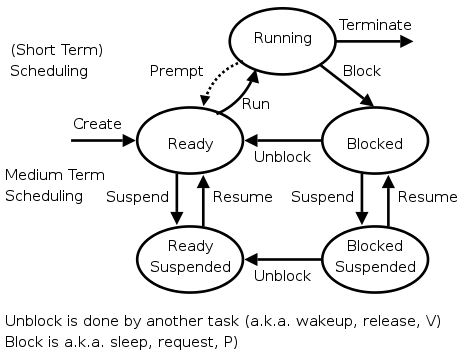
\includegraphics[width=0.6\textwidth]{./figure/scheduling.png}
      \caption{Operating System Scheduler \cite{sched}}
       \label{scheduler}
\end{figure}



\subsection{Scheduling Precision}
To understand the performance impact of utilizing Docker containers for software deployment, the experiment conducted in this study will analyse the scheduling precision and input/output performance of the automotive real-time application. The application executes time-triggered computations within elements referred to as time-slices. The time-slice is a specification of time allocated for the algorithm to execute and deliver a result. A real-time application running at \texttt{100 hertz} executes 100 time-slices per second, which results in one time-slice being \texttt{10 milliseconds} or \texttt{0.01 second}. The \texttt{10 milliseconds} time-slice is the time deadline set for the specific application, which is the maximum time allowed for the assigned algorithm to finish its computations. In scenarios where the algorithm utilises less than the assigned time-slice the application will sleep for the remaining time until it fires a new execution. The operating system scheduler is responsible for assuring that the application sleeps for the time specified by the real-time application. The scheduler is also responsible for waking the real-time process after the specified sleeping time has elapsed. Other than the assigned algorithm, the real-time application consists of code which is responsible for communicating with the OS scheduler that controls the sleep of the time-slices. Therefore a part of the time-slice has to be consumed to execute the required code. The time consumed by the code which controls the sleep of the application is referred to as the middle-ware overhead which is part of what is used for measuring the scheduling precision of the execution environments specified in the experiment of this study.\\

Scheduling precision refers to how accurately the application executes the specified algorithm from the point of firing the time-slice until the algorithm begins its computation. Further accuracy is measured between the point of where the algorithm finishes its computations until the real-time application sleeps. Lastly, measurements are done to see whether the \texttt{sleep} function of the system actually sleeps for the remainder of the time-slice or if it overstays the specified timing deadline.\\

The limitations of each execution environment utilised in the experiment of this study can be identified by understanding how much time each part of the required code occupies the time-slice. The less time required for executing the code outside of the assigned algorithm the more deterministic a system is said to be. In a scenario where the assigned algorithm requires 80\% of the time-slice to execute the code, it is assumed that the application will sleep for the remaining 20\%. However, as there exists additional operations surrounding the algorithm the application might sleep 18\% whereas 2\% is required for the surrounding code to execute. If the application still sleeps 20\%, executes the algorithm for 80\%, and uses 2\% for the required code it will overstay its time-slice by 2\% thus rendering the application less deterministic (by a small amount). It is the time available for the algorithm the experiments of this study will seek to identify to inform software engineers of how much of the time-slice can be used for effective computations, i.e. time available for generating a result.

\subsection{Preemptive Scheduling}
A general purpose operating system scheduler, such as the scheduler found in Ubuntu Linux 14.04, implements a FIFO (first-in-first-out) approach with two process scheduler algorithms. Namely, a time-sharing algorithm and a real-time algorithm where the former is a scheduler that maintains fairness, distributing the system's resources equally over all processes in the queue ensuring that no process is completely starved. The later is an algorithm which prioritises the processes based on their set importance, where a higher prioritised process is provided more resources in comparison with a lower process. However, the generic Linux kernel version does not allow the scheduler to cancel all resources for processes already utilising the CPU. A higher prioritised process will therefore not be able to utilise 100\% of the CPU's resources if there are other processes already using the CPU. For a general purpose operating system this approach is standard practise and is logical for non time critical processes. However for a real-time system it is crucial to ensure that the highest level process can interrupt any running processes at any point in time and occupy all resources available to ensure the process meets the time deadline. A real time enabled kernel using the RT\_preempt kernel patch implements the preemptive approach thus allowing for such a behaviour of cancelling resources from lower prioritised processes to occupy all resources for a time-sensitive high priority process. Furthermore, the RT\_preempt patch applies resource locking for RT prioritised processes so that lower prioritised processes cannot utilise the same resource simultaneously.

%An operating system handles the communication between the software and the hardware, more specifically the operating system kernel acts as the interface between hardware and software. As an operating system is running a vast amount of processes simultaneously there is a need to prioritise and select which processes to run at what time. Each process utilises the CPU to make the computations required for the process to operate. The CPU is a powerful piece of hardware which can handle the same number of processes as it has cores and threads, i.e. an general Intel Core i7 processor has 4 cores and two threads per core amounting to 8 total processes simultaneously. However an operating system may run more processes than the CPU can process simultaneously. To manage this flood of processes a software component referred to as the \textit{CPU scheduler} which is configured by the kernel and is implemented to ensure that there is a queuing system set up for all processes running on the system. 

%---------------------------------------------------%
\section{Software Deployment}
%Software deployment for CPS is difficult as there are many aspects to put into consideration. Typically,  CPS are resource constrained, meaning that you cannot scale up hardware exponentially as you typically do not have the physical space for it. Secondly, real-time requirements are needed, so any SD tools needs to be lightweight. Finally, there are safety concerns since CPS typically interact with their surroundings. 

Software deployment is a crucial part of the software development, it refers to the activities which makes the software system available for use \cite{carzaniga1998characterization}. The process contains a number of activities which all play into the life cycle of a software system with the goal to implement into the runtime environment where the system is set to operate live. These activities are namely: \\

\textbf{Release} – is the activity of packaging the software for delivering it to the end user. This includes processes such as including the software's requirements and dependencies to external components, such as libraries and applications. It also includes the process of advertising – the process of informing interested parties about the software being released.\\
\textbf{Install} – refers to the activities of assembling all required resources for the runtime environment. It consists of two specific process, namely \textit{transfer} and \textit{configuration}. Where the former is the process of transferring the software from the developer to the runtime environment and the later is the process of making the software ready for activation.\\
\textbf{Activate} – is the process of executing the software and all dependent applications in the runtime environment.\\
\textbf{Deactivate} – is the opposite of the \textit{activate} activity.\\
\textbf{Update} – is the activity of updating the version of the running software which consists of similar activities of the \textit{install} activity.\\
\textbf{Adapt} – refers to the process of ensuring that the updated version is running correctly in the runtime environment.\\
\textbf{Deinstall} – is the activity of decommissioning the running software and includes sub-activities such as removing the external libraries and components.\\
\textbf{Derelease} – is the final activity which includes the process of advertising the withdrawal of the software system.\\

All these activities differ in how they are executed depending on the software engineering paradigm utilised for the software project. Traditional software engineering practices, e.g. the waterfall model, seeks to execute the software deployment process at the end of the software's development cycle. Whereas more novel software engineering practices aim to execute the software deployment process continuously throughout the software's development cycle. In state-of-art software engineering practices such as continuous integration and continuous deployment, software is required to be deployed daily \cite{meyer2014continuous} for full adaptation. Such requirements can easily make the process of software deployment exhausting and complex, where software tools such as Docker would simplify these processes greatly. Docker simplifies processes found within each of the software deployment activities, as it provides the runtime environment before the software deployment process has begun. The development environment is a clone of the production environment thus transferring the deployment processes from the live production server to a confined secure location where the deployment process does not affect the usability of the current running software.\\


\begin{figure}[ht]
\centering
     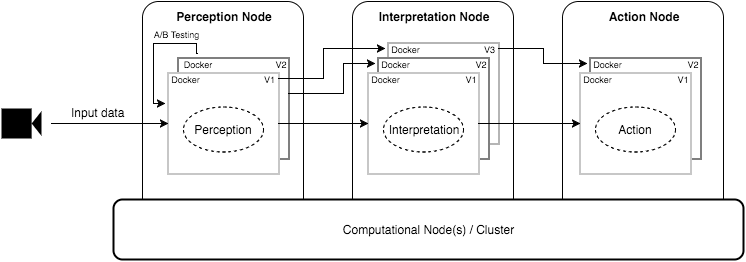
\includegraphics[width=1.0\textwidth]{./figure/containers.png}
      \caption{Run-time environment using Docker.}
       \label{containers}
\end{figure}

Figure \ref{containers} exemplifies a deployment strategy design utilising Docker in the context of self-driving vehicles. The responsibilities are broken down into three computational nodes in which Docker containers are running instances of the code base independently. Each Docker container can run different versions of the separate nodes, where the interpretation node has three versions running separately. Version one (denoted V1) in each node represents the latest working configuration while other versions are run to test code which is still under development. Having multiple versions of a running environment allows for safe and simple roll-backs in the event of buggy code or degraded performance. Furthermore, multiple versioning of the same Docker container allows for split testing between different containers to take place. With an always functioning configuration, the development team can demonstrate a functioning version of the product to stakeholders at any point in the development cycle. The ability to demonstrate the product at any point in the development phase adds to the business value of the project, as possible investors or stakeholders can be presented a functioning product although the product is currently under development. This is possible with current deployment approaches, however the implementation of cloning systems or running virtual machines is more resource demanding \cite{vmvscontainers} and not as flexible in comparison with utilising Docker for the deployment strategy.


%---------------------------------------------------%
\section{Container-Based Virtualization}
%process isolation and application portability
%virtualization can be done with fully-fledged Virtual Machines or lightweight containers. VMs  incure higher ovhead but better protection and so are not suitable for autonomous vehicles.  Therefore we adopt containers and strive to minimize latency by real-time Linux kernel
%containers very efficiently share and utilize CPU and memory resources, 
% !!! Add in Dockerhub

Docker is an open source light-weight container environment which was initially launched in 2013 and has gained ground rapidly with its simplicity. The environment offered by Docker simplifies the process of software deployment by packaging all dependencies into a light-weight virtualization container which ensures that all instances of the software is utilising the same dependent libraries. The functionality provided by Docker is comparable with virtual machines as both are virtualised environments where software applications can be executed with all dependent libraries and applications installed. However, Docker, in contrast to virtual machines, is a light-weight alternative as it communicates directly to the host machine's kernel. A virtual machine applies the additional levels of a virtual operating system which adds complexity and does not speak directly with the host machine's kernel. With the benefit of packaging the dependent libraries and applications into a container, software developers can avoid uncertain deployments where library versions may differ between the developers' development environments and the live production environment. Docker presents further benefits such as safe roll-back between different software versions which provides projects the ability to always be able to fall back on application versions which are known to function correctly. By providing these benefits project managers can feel secure in that there always exists a working runtime environment in the scenario of a new failing deployment.\\

The container in which Docker packages all dependent libraries and applications are referred to as a Docker image. This image contains everything which is required for an application to be executed. In the case of self-driving vehicles such dependencies may be image processing libraries such as OpenCV and the middle ware which enables the real-time application. When executing an application within Docker, a container is generated and executed based on the Docker image which consists of the installed libraries and applications. This software design allows for split testing of software as the same application can be executed multiple times without clashing with the other contained application. Thus being optimal for testing different versions of the same application simultaneously while knowing there is no interference between the executed applications.

%---------------------------------------------------%